\documentclass[12pt,a4paper]{article}
\usepackage[utf8]{inputenc}
\usepackage{amsmath}
\usepackage{amsfonts}
\usepackage{amssymb}
\usepackage{graphicx}
\usepackage[left=2cm,right=2cm,top=2cm,bottom=2cm]{geometry}
\usepackage{float}
\usepackage{hyperref}
\usepackage[T1]{fontenc}
\usepackage[polish]{babel}
\usepackage[utf8]{inputenc}
\usepackage{caption}
\usepackage{subcaption}

\author{Maciej Kajdak\\nr indeksu: 226256}
\title{Sprawozdanie 2 \\ \textbf{Modelowanie i identyfikacja}}
\renewcommand{\thesection}{\arabic{section}}

\begin{document}
\maketitle
\section{Wstęp}
Empriyczne wyznaczanie własności pewnych sygnałów, które przypuszczalnie rządzą się prawami pewnego nieznanego rozkładu jest zadaniem, które stawiane jest przy problemach identyfikacji systemów.
Dzięki poprawnemu zidentyfikowaniu obiektu, który się obserwuje można przewidywać jego zachowania, a następnie odpowiednio taką wiedzę wykorzystywać.

W tym celu potrzebne jest narzędzie -- estymator, pozwalający na wyznaczenie a następnie weryfikowanie poprawności przypuszczeń.
W niniejszym sprawozdaniu opisano przebieg badań estymatorów pewnych rozkładów prawdopodobieństwa i ich własności.
Większość badań została przeprowadzona w środowisku Python w wersji 3.7.1 \cite{python3} wraz z pakietami numpy w wersji 1.15.4 \cite{numpy} oraz matplotlib w wersji 3.0.2 \cite{matplotlib}.
Wszystkie stworzone w ramach laboratoriów skrypty można znaleźć w \href{https://github.com/MacAndKaj/Modeling\_and\_Identification}{\underline{repozytorium twórcy w serwisie Github}}

\section{Podstawy estymacji}
W celu wyznaczenia cech jakimi charakteryzuje się ciąg zmiennych losowych można posłużyć się empirycznymi metodami wyznaczania estymatorów.
Do badania cech estymatorów wygenerowano ciąg zmiennych losowych o rozkładzie normalnym $\mathcal{N}(0,1)$.

\subsection{Estymatory empiryczne}
Na podstawie wygenerowanych próbek wyznaczono wartości $\hat{\mu}_{N}$, obliczanego przy pomocy wyrażenia \ref{eq:estymatorWartOczek}, w funkcji N.
Następnym krokiem było wyznaczenie estymatorów wariancji obciążonej (wyrażenie \ref{eq:estymatorVarO} oraz nieobciążonej \ref{eq:estymatorVarNO}.
Sprawdzano w ten sposób jaki wpływ na jakość estymacji wartości oczekiwanej oraz wariancji ma ilość wygenerowanych próbek.
Wyniki badań jako funkcje poszczególnych estymatorów od x przedstawiono na rysunku \ref{fig:estymatory}.
W ten sam sposób wyznaczono estymatory dla rozkładu Cauchyego, zostały one przedstawione na rysunku \ref{fig:estymatoryCauchy}.
Dla rozkładu normalnego estymatory w miarę zwiększania ilości badanych próbek stabilizują się na właściwych wartościach, tzn na $\mu=0$ oraz $\sigma^{2}=1$.
Z kolei dla rozkładu Cauchy'ego wyznaczanie estymatorów kończy się ogromnymi błędami.
Jest to spowodowane faktem, że rozkład Cauchy'ego nie ma ani wartości średniej ani wariancji, więc wynik eksperymentu był oczekiwany.


\begin{equation}\label{eq:estymatorWartOczek}
\hat{\mu}_{N} = \frac{1}{N}\sum_{n=1}^{N}X_{N}
\end{equation}

\begin{equation}\label{eq:estymatorVarO}
\hat{s}^{2}_{N} = \frac{1}{N}\sum_{n=1}^{N}(X_{N}-\hat{\mu}_{N})
\end{equation}

\begin{equation}\label{eq:estymatorVarNO}
\hat{S}^{2}_{N} = \frac{1}{N-1}\sum_{n=1}^{N}(X_{N}-\hat{\mu}_{N})
\end{equation}

\begin{figure}[H]
\centering
\includegraphics[width=\textwidth]{../Obrazy/Spr2/estymatoryNormalny.png} 
\caption{Wykresy estymatorów empirycznych w funkcji N dla rozkładu normalnego}
\label{fig:estymatory}
\end{figure}

\begin{figure}[H]
\centering
\includegraphics[width=\textwidth]{../Obrazy/Spr2/estymatoryCauchy.png} 
\caption{Wykresy estymatorów empirycznych w funkcji N dla rozkładu Cauchy'ego}
\label{fig:estymatoryCauchy}
\end{figure}

\subsection{Błąd empiryczny}
Aby udowodnić poprawność i skuteczność działania estymatorów empirycznych można posłużyć się wskaźnikiem wyznaczającym błąd empiryczny.
Jest on definiowany wzorem \ref{eq:bladu} oraz analogicznie dla wariancji obciążonej (\ref{eq:blads}) i nieobciążonej (\ref{eq:bladS}).

\begin{equation}\label{eq:bladu}
Err\{\hat{\mu}_{N};\mu\}=\frac{1}{L}\sum\limits_{l=1}^{L}\Big[\hat{\mu}_{N}^{[l]}-\mu\Big]
\end{equation}

\begin{equation}\label{eq:blads}
Err\{\hat{s}_{N};\mu\}=\frac{1}{L}\sum\limits_{l=1}^{L}\Big[\hat{s}_{N}^{[l]}-s\Big]
\end{equation}

\begin{equation}\label{eq:bladS}
Err\{\hat{S}_{N};\mu\}=\frac{1}{L}\sum\limits_{l=1}^{L}\Big[\hat{S}_{N}^{[l]}-S\Big]
\end{equation}

\begin{figure}[H]
\centering
\includegraphics[width=\textwidth]{../Obrazy/Spr2/bladNormalny.png} 
\caption{Wykresy błędów estymatorów dla rozkładu normalnego.}
\label{fig:bladNormalny}
\end{figure}

\section{Dystrybuanta empiryczna i jej własności}
W celu przebadania własności estymatora dystrybuanty empirycznej wygenerowano ciąg liczb losowych przy pomocy wcześniej zaimplementowanego generatora. 
Gęstość rozkładu prawdopodobieństwa, z którego generowane były liczby przedstawiono w postaci równania \ref{eq:rozkladDowolny}. 
W wyniku generacji otrzymano ciąg liczb losowych $\{X_{1},X_{2},\dots,X_{N}\}$.

\begin{equation}\label{eq:rozkladDowolny}
f(x) = \begin{cases} 2x, & \mbox{dla } x \in [0,1] \\ 0, & \mbox{dla } x \in (-\infty,0) \cup (1,\infty) \end{cases}
\end{equation}

Dla tak wygenerowanego przebiegu wyznaczono dystrybuantę empiryczną zaimplementowaną w postaci \ref{fig:dystrybuantaEmpiryczna}. Wykresy dystrybanty empirycznej dla różnych wartości N przedstawiono na rysunku \ref{fig:dystrybuantaEmpiryczna}.
Jak można się było spodziewać, dla małej ilości próbek dystrybuanta nie działa dobrze, jednak wraz ze wzrostem ilości próbek dystrybuanta empiryczna coraz bardziej przypomina rzeczywisty przebieg. 

\begin{equation}\label{eq:dystrybuantaEmpiryczna}
\hat{F}_{N}(x)=\frac{1}{N}\sum^{N}_{n=1}\textbf{I}(X_{n} \le x)
\end{equation}
, gdzie
\begin{equation}
\textbf{I}(a \le b) = \begin{cases} 1 &\iff a \le b \\ 0 &\iff a > b \end{cases} 
\end{equation}

\begin{figure}[H]
\centering
\includegraphics[width=--\textwidth]{../Obrazy/Spr2/dystrybuantaEmpirycznaWykresy.png} 
\caption{Wykresy dystrybuanty empirycznej na tle prawdziwego przebiegu dystrybuanty dla różnej wartości N}
\label{fig:dystrybuantaEmpiryczna}
\end{figure}

Tak tworzona dystrybuanta empiryczna może również zostać poddana testom sprawdzającym jej wiarygodność, tzn. czy dystrybuanta empiryczna faktycznie przebiegiem przypomina tę poszukiwaną.
Można do tego celu wykorzystać wskaźnik przedstawiany wyrażeniem \ref{eq:kolmogorov}.
Mówiąc ściślej, badanie jakości dystrybuanty empirycznej takim wskaźnikiem nazywane jest \textit{testem Kołmogorowa}.
Bada on różnice między hipotetyczną dystrybuantą $F$ a dystrybuantą empiryczną $\hat{F}_{N}$.
Dla omawianego problemu wyznaczono taki wskaźnik i przedstawiono go na rysunku \ref{fig:bladDystrybuanty} w zależności od liczby próbek.
Na pierwszy rzut oka widać jak wielki wpływ ma ilość próbek na jakość estymacji, ponieważ wraz ze wzrostem poziomu wiedzy o wyjściu systemu generującego przebieg o takiej dystrybuancie zmniejsza się błąd, a tym samym można przypuszczać, że dystrybuanta empiryczna wyznaczana jest poprawnie, a generowane liczby faktycznie pochodzą z pożądanego rozkładu.


\begin{equation}\label{eq:kolmogorov}
D_{N}=\sup_{x}|\hat{F}_{N}(x)-F(x)|
\end{equation}

\begin{figure}[H]
\centering
\includegraphics[width=\textwidth]{../Obrazy/Spr2/blad.png} 
\caption{Błąd dystrybuanty empirycznej}
\label{fig:bladDystrybuanty}
\end{figure}

\subsection{Badanie nieznanej próby}
W celu sprawdzenia sposobu działania dystrybuanty empirycznej wykorzystano ciąg liczb losowych pochodzący z nieznanego rozkładu prawdopodobieństwa.
Aby określić z z jakiego rozkładu mogą pochodzić próbki wyznaczono dystrybuantę empiryczną oraz przetestowano estymator pod kątem trzech hipotetycznych rozkładów: $\mathcal{N}(1,1)$, $\mathcal{N}(0,5)$ oraz Cauchy'ego z parametrami $x_{0}=0$ oraz $\gamma=1$.
Na rysunkach \ref{fig:normal11}, \ref{fig:normal11}, \ref{fig:normal11} przedstawiono przebiegi estymatora na tle dystrybuant ww. rozkładów oraz błąd w zależności od ilości wziętych próbek.
Na tej podstawie można wnioskować, że najprawdopodobniej próbki pochodzą z rozkładu Cauchy'ego.

\begin{figure}[H]
\centering
\includegraphics[width=\textwidth]{../Obrazy/Spr2/normal11.png} 
\caption{Porównanie dystrybuanty empirycznej z rozkładem normalnym (1,1)}
\label{fig:normal11}
\end{figure}

\begin{figure}[H]
\centering
\includegraphics[width=\textwidth]{../Obrazy/Spr2/normal05.png} 
\caption{Porównanie dystrybuanty empirycznej z rozkładem normalnym (0,5)}
\label{fig:normal05}
\end{figure}

\begin{figure}[H]
\centering
\includegraphics[width=\textwidth]{../Obrazy/Spr2/cauchy01.png} 
\caption{Porównanie dystrybuanty empirycznej z rozkładem Cauchy'ego (0,1)}
\label{fig:cauchy01}
\end{figure}

\subsection{Estymator wariancji dystrybuanty empirycznej}
Do wyznaczenia wariancji dystrybuanty empirycznej wykorzystano fakt, że wariancja jest kwadrat różnicy między próbką z dystrybuanty empirycznej a wartością oczekiwaną rzeczywistej dystrybuanty.
Dla rozkładu \ref{eq:rozkladDowolny} wykres wariancji dystrybuanty empirycznej przedstawiono na rysunku.
Z tego co przedstawia wykres można wnioskować, że najtrudniejsza estymacja dystrybuanty jest tam, gdzie zmiany przebiegu są coraz większe stąd większy rozrzut próbek wokół wartości oczekiwanej -- na wykresie widoczne zwiększenie wariancji.


\begin{equation}\label{eq:wariancja}
\sigma^{2}_{F}(x) = (\hat{F}_{N}(x)-F(x))^{2}
\end{equation}

\begin{figure}[H]
\centering
\includegraphics[width=\textwidth]{../Obrazy/Spr2/estymatorWariancji.png} 
\caption{Wykres wariancji dystrybuanty empirycznej}
\label{fig:wariancja}
\end{figure}



\section{Centralne twierdzenie graniczne}
Jednym z ważniejszych twierdzeń w teorii probabilistyki jest właśnie centralne twierdzenie graniczne, ponieważ uzasadnia ono, dlaczego w przyrodzie tak wiele losowych elementów rządzi się rozkładem normalnym.
Generując ciągle próbki o tej samej wartości oczekiwanej oraz tej samej wariancji stale zwiększając liczbę wygenerowanych próbek można zaobserwować, że histogram próbek coraz bardziej przypominać będzie rozkład normalny.
Wykres przedstawiony na rysunku \ref{fig:ctg} przedstawia kolejne generowane ciągi próbek o tej samej wariancji i wartości oczekiwanej. 
Jak można zauważyć coraz mocniejsza żółć środkująca się w poziomie oznacza, że histogram generowanych próbek zbiega do rozkładu normalnego.
Lepiej można ten proces zauważyć na rysunkach , które są przekrojami wykresu z rysunku \ref{fig:ctg} z początku, połowy i końca generowania kolejnych prób.
Wraz ze wzrostem wygenerowanych próbek rozkład budowany na ich podstawie coraz zbiega do rozkładu normalnego.

\begin{figure}[H]
\centering
\includegraphics[width=.8\textwidth]{../Obrazy/Spr2/ctg.png} 
\caption{Wykres kształtu rozkładu normalnego w zależności od liczby wygenerowanych próbek}
\label{fig:ctg}
\end{figure}


\begin{figure}
\centering
\begin{subfigure}{.3\textwidth}
    \centering
   	\includegraphics[width=\textwidth]{../Obrazy/Spr2/ctg1.png} 
\end{subfigure}%
\begin{subfigure}{.3\textwidth}
  	\centering
	\includegraphics[width=\textwidth]{../Obrazy/Spr2/ctg2.png} 
\end{subfigure}
\begin{subfigure}{.3\textwidth}
  	\centering
	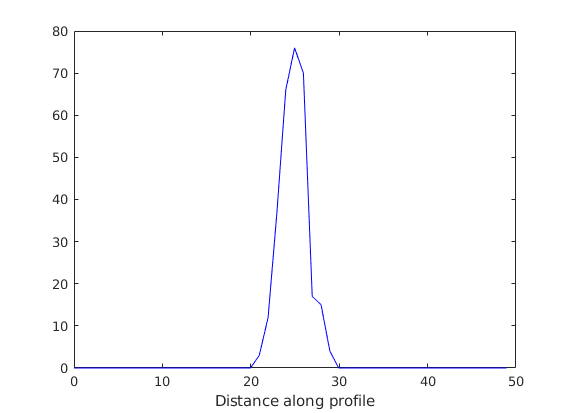
\includegraphics[width=\textwidth]{../Obrazy/Spr2/ctg3.png} 
\end{subfigure}
\caption{A figure with two subfigures}
\label{fig:test}
\end{figure}



\section{Jądrowy estymator gęstości prawdopodobieństwa}
Podczas identyfikowania systemów pojawia się zadanie zbadania tego jaki rozkład prawdopodobieństwa może przedstawiać badany ciąg liczb losowych. Aby to sprawdzić potrzebne jest narzędzie, które mogłoby odtwarzać ten rozkład.
Do tego celu może posłużyć jądrowy estymator gęstości prawdopodobieństwa.
Wyraża się on jako równanie \ref{eq:jadrowyEstymator}, gdzie $K(\cdot)$ jest jądrem estymatora.

Do badań ww.\ estymatora wykorzystano próbę o liczności $N=500$ wygenerowaną z rozkładu normalnego $\mathcal{N}(1,1)$ 

\begin{equation}\label{eq:jadrowyEstymator}
\hat{f}_{N}(x)=\frac{1}{Nh_{N}}\sum^{N}_{n=1}K\bigg(\frac{X_{n} - x}{h_{N}}\bigg)
\end{equation}

\subsection{Jądro prostokątne}
Jedną z najprostszych funkcji jądrowych jest jądro prostokątne. 
Wyraża się ono jako równanie \ref{eq:jadroProstokatne}.
Wykorzystane zostało do wyznaczenia estymatora jądrowego dla wygenerowanych próbek.
Jak widać do wyznaczania jądrowego estymatora gęstości prawdopodobieństwa potrzebny jest parametr $h$ nazywany parametrem wygładzania.
Na rysunku \ref{fig:jadrowyProstokatny} przedstawiono wykresy z wyznaczonym estymatorem dla różnych wartości parametru $h$ co obrazuje jaki wpływ na estymator ma ww. parametr.
Co więcej, na podstawie przebiegów można wnioskować, że dla takiego problemu optymalna wartość parametru wygładzania znajduje się gdzieś w przedziale $(0.25,1)$

\begin{equation}\label{eq:jadroProstokatne}
\textbf{I}(x) = \begin{cases} \frac{1}{2} &,dla\ |x| \le 1 \\ 0 &,dla\ |x|>1 \end{cases} 
\end{equation}

\begin{figure}[H]
\centering
\includegraphics[width=\textwidth]{../Obrazy/Spr2/jadrowyProstokatny.png} 
\caption{Jądrowy estymator gęstości prawdopodobieństwa na tle prawdziwego przebiegu dla kilku różnych wartości parametru wygładzania.}
\label{fig:jadrowyProstokatny}
\end{figure}

Oczywiście wybór odpowiedniego jądra estymatora również jest kwestią podyktowaną doborem najlepszego z możliwych narzędzi.
Oprócz jądra prostokątnego przetestowano także jądro gaussowskie, Epanecznikowa, cosinusowe oraz tricube.
Przebiegi wyznaczonych esteymatorów w funkcji x przedstawiono na rysunku \ref{fig:jadra}.
Jak można się było spodziewać dość dobrym estymatorem rozkładu normalnego jest estymator oparty na jądrze gaussowskim.
Jednak jądro Epanecznikowa również bardzo dobrze dopasowuje się do przebiegu funkcji gęstości rozkładu normalnego, podobnie jądro cosinusowe.
Co więcej jądro Epanecznikowa i jądro Cosinusowe są mniej zależne od parametru h, co sprawdzono badając ich przebiegi dla kilku różnych wartości parametru wygładzania co może potwierdzać ich dość dobre własności. 

\begin{figure}[H]
\centering
\includegraphics[width=\textwidth]{../Obrazy/Spr2/jadra.png} 
\caption{Estymatory gęstości prawdopodobieństwa dla różnych funkcji jądra.}
\label{fig:jadra}
\end{figure}

Takim samym badaniom poddano próbki wygenerowane z rozkładu trójkątnego.
Wyniki eksperymentów przedstawiono na rysunku \ref{fig:trjkatny}.
W tym przypadku widać, że jądro Epanechnikowa oraz jądro cosinusowe radzą sobie najlepiej.
Jądro Gaussa prawdopodobnie poradziłoby sobie lepiej, gdyby odszukać odpowiedni współczynnik wygładzania.

\begin{figure}[H]
\centering
\includegraphics[width=\textwidth]{../Obrazy/Spr2/trojkatnyEstymator.png} 
\caption{Estymatory jądrowe dla próbek pochodzących z rozkładu trójkątnego.}
\label{fig:trjkatny}
\end{figure}

\subsection{Błąd empiryczny}
Dla wyznaczanego metodą empiryczną rozkładu można zdefiniować błąd empiryczny, tj. błąd jaki generowany jest podczas estymowania prawdziwego rozkładu, definiowany jako różnica między estymatorem a wartością rozkładu dla danej wartości wejściowej.
Błąd empiryczny definiowany jest w postaci wyrażenia \ref{eq:bladEmpiryczny}.
Dla wyżej analizowanego rozkładu wyznaczony błąd empiryczny przedstawiono na rysunku \ref{fig:bladEmpiryczny}.
W ten sposób można zauważyć, że parametr h przyjmuje optymalną wartość w okolicach 0.2--0.4 jednak, aby stwierdzić to dokładnie, należałoby zbadać pod kątem podobieństwa rozkładów dla parametru wygładzania z tego przedziału.

\begin{equation}\label{eq:bladEmpiryczny}
Err\{\hat{f}_{N}\}=\frac{1}{LM}\sum_{l=1}^{L}\sum_{m=1}^{M}\Big[\hat{f}^{[l]}_{N}(x_{m})-f(x_{m})\Big]^{2}
\end{equation}

\begin{figure}[!h]
\centering
\includegraphics[width=.8\textwidth]{../Obrazy/Spr2/bladEmpiryczny.png} 
\caption{Błąd empiryczny dla próby pochodzącej z rozkładu normalnego w zależności od parametru wygładzania h}
\label{fig:bladEmpiryczny}
\end{figure}

\section{Jądrowy estymator funkcji regresji}
Innym sposobem modelowania nieznanych rozkładów prawdopodobieństwa jest jądrowy estymator funkcji regresji.
Również on wykorzystuje w swoim działanie funkcję będącą jądrem estymatora.


\subsection{Estymator dla systemu nieliniowego}
Tym razem do przeprowadzenia badań przyjęto, że system nieliniowy ma charakterystykę $m(x)=tan(x)$. Wejściem systemu są próbki sygnału losowego posiadającego równomierny rozkład prawdopodobieństwa $\mathcal{U}(-2,2)$, a wyjście obiektu jest poddane zakłóceniom działającym na wyjście z gęstością rozkładu normalnego $\mathcal{N}(0,0.5)$.
Wykres przedstawiający zależność wyjścia od wejścia obiektu (chmura punktów -- Y(x)) została przedstawiona na rysunku \ref{fig:system}. 
Został on przedstawiony na tle rzeczywistego przebiegu wyjścia bez zakłóceń.

\begin{figure}[H]
\centering
\includegraphics[width=\textwidth]{../Obrazy/Spr2/system.png} 
\caption{Wyjście systemu w zależności od jego wejścia}
\label{fig:system}
\end{figure}

Jak widać na wykresie chmura punktów układa się w pożądanym kształcie, jednak zakłócenia, którym poddany jest sygnał wyjściowy 'rozmywa' w znaczący sposób dane wyjściowe.
W takim wypadku można skorzystać z estymatora, który na podstawie takiej chmury mógłby wyznaczyć przypuszczalnie prawdziwy przebieg odpowiedzi systemu.
Jądrowy estymator funkcji regresji wyraża się równaniem \ref{eq:estymatorRegresji}.
Do badań przyjęto, że jądrem estymatora będzie jądro prostokątne.
Sprawdzano różnice w działaniu estymatora dla kilku wartości parametru wygładzania, wyniki zostały przedstawione na rysunku \ref{fig:estymatorRegresji}.
Ponownie widać, że pewna optymalna wartość parametru wygładzania znajduje się w okolicach $h_{N}=0.5$.

\begin{equation}\label{eq:estymatorRegresji}
\hat{m}_{N}(x)=\frac{\sum\limits^{N}_{n=1}Y_{n}K\bigg(\frac{X_{n} - x}{h_{N}}\bigg)}{\sum\limits^{N}_{n=1}K\bigg(\frac{X_{n} - x}{h_{N}}\bigg)}
\end{equation}

\begin{figure}[H]
\centering
\includegraphics[width=\textwidth]{../Obrazy/Spr2/estymatorRegresji.png} 
\caption{Estymator funkcji regresji dla kilku wybranych wartości parametru wygładzania}
\label{fig:estymatorRegresji}
\end{figure}


W celu sprawdzenia wpływu doboru jądra estymatora na jakość działania estymatora wykorzystano poprzednio używane jądra.
Ustalając parametr wygładzania na poziomie $h_{N}=0.6$ wyznaczono estymator w funkcji x dla 4 różnych jąder.
Wyniki estymacji przedstawiono na rysunku \ref{fig:regresjiJadra}.
Ponownie jądro Epanecznikowa oraz cosinusowe niezwykle dobrze dopasowuje estymator do rzeczywistego przebiegu.
W podobny sposób sprawdzono wpływ parametru $a$(będącego parametrem obiektu), czyli kształt nieliniowości, na jakość estymatora.
Na rysunku \ref{fig:regresjaNieliniowosc} przedstawiono 4 wykresy pokazujące jak estymator jądrowy funkcji regresji, oparty o jądro Epanecznikowa z parametrem wygładzania $h_{N}=0.5$, zmienia swoją jakość w zależności od stopnia nieliniowości obiektu.
Jak widać, estymator traci wydajność im bardziej charakterystyka 'przyspiesza' swoje zmiany.

\begin{figure}[H]
\centering
\includegraphics[width=\textwidth]{../Obrazy/Spr2/jadraRegresja.png} 
\caption{Estymatory funkcji regresji używające różnych jąder: funkcja jądra Gaussa, jądra Cosinusowego, Epanecznikowa oraz prostokątnego}
\label{fig:regresjiJadra}
\end{figure}


\begin{figure}[H]
\centering
\includegraphics[width=\textwidth]{../Obrazy/Spr2/regresjaNieliniowosc.png} 
\caption{Estymatory funkcji regresji dla różnego stopnia nieliniowości obiektu.}
\label{fig:regresjaNieliniowosc}
\end{figure}

\subsection{Optymalna wartość parametru wygładzania}
Jako, że parametr wygładzania nie ma pewnej stałej, można próbować optymalizować jego wartość pod kątem jakości estymacji, czyli różnicy pomiędzy estymatorem a estymowanym rozkładem.
Do tego celu może posłużyć funkcja wyrażona równaniem \ref{eq:validH}.
Wartości błędu w zależności od parametru wygładzania został przedstawiony na rysunku \ref{eq:validH}.
Na tej podstawie wyznaczono optymalną wartość parametru h dla 4 różnych jąder estymatora.
Wyniki badań przedstawiono na rysunkach \ref{fig:optBoxcar}, \ref{fig:optGauss}, \ref{fig:optEpanechnikov}, \ref{fig:optCosine}.

\begin{equation}\label{eq:validH}
valid(h)=\frac{1}{2Q}\sum\limits_{q=-Q}^{Q}\bigg[\hat{m}_{N}\bigg(\frac{q}{Q}\bigg)-m\bigg(\frac{q}{Q}\bigg)\bigg]^{2}
\end{equation}

\begin{figure}[H]
\centering
\includegraphics[width=.8\textwidth]{../Obrazy/Spr2/optBoxcar.png} 
\caption{Wykres $valid(h)$ oraz estymator oparty o jądro prostokątne dla tak wybranego parametru wygładzania.}
\label{fig:optBoxcar}
\end{figure}

\begin{figure}[H]
\centering
\includegraphics[width=.8\textwidth]{../Obrazy/Spr2/optGauss.png} 
\caption{Wykres $valid(h)$ oraz estymator oparty o jądro Gaussa dla tak wybranego parametru wygładzania.}
\label{fig:optGauss}
\end{figure}

\begin{figure}[H]
\centering
\includegraphics[width=.8\textwidth]{../Obrazy/Spr2/optEpanechnikov.png} 
\caption{Wykres $valid(h)$ oraz estymator oparty o jądro Epanecznikowa dla tak wybranego parametru wygładzania.}
\label{fig:optEpanechnikov}
\end{figure}

\begin{figure}[H]
\centering
\includegraphics[width=.8\textwidth]{../Obrazy/Spr2/optCosine.png} 
\caption{Wykres $valid(h)$ oraz estymator oparty o jądro cosinusowe dla tak wybranego parametru wygładzania.}
\label{fig:optCosine}
\end{figure}

\subsection{Zakłócenia z rozkładem Cauchy'ego}
Badania zostały również przeprowadzone dla zakłóceń generowanych z rozkładem Cauchy'ego co oznacza, że nie miały one pewnej stałej wartości oczekiwanej oraz wariancji.
Wykres wartości na wyjściu obiektu przedstawiony został na rysunku \ref{fig:cauchyDist}.
Jak można przypuszczać, dalekie odchyłki niektórych próbek mogą powodować nieprawidłowe działanie estymatora.
Wygenerowane estymatory dla różnych jąder estymatora z parametrem wygładzania $h_{N}=0.5$ zostały przedstawione na rysunku \ref{fig:bladCauchyDist}.
Wykresy potwierdzają przypuszczenia -- rzadkie, lecz wielkie odchyłki od wartości oczekiwanej powodują, że estymator nie działa wystarczająco dobrze.
Jedynie jądro gaussowskie dość dobrze estymuje prawdziwy przebieg, dlatego też w kolejnym badaniu zmianie ulegał parametr wygładzania.
Wyniki badań przedstawiono na rysunku \ref{fig:bladCauchyDistParam}.
Jak widać odpowiednie dobranie parametru wygładzania kompensuje problemy z szumem zakłócającym sygnał.
Ostatnim eksperymentem, było badanie zachowania estymatora w zależności od zmieniającego się parametru a.
Wynik został przedstawiony na rysunku \ref{fig:bladCauchyDistNielin}.
Ponownie widać, że wraz ze zmieniającą się nieliniowością estymator traci swoje właściwości.

\begin{figure}[H]
\centering
\includegraphics[width=.8\textwidth]{../Obrazy/Spr2/cauchyDist.png} 
\caption{Wykres wyjściowy obiektu zaszumiony zakłóceniami o rozkładzie Cauchy'ego.}
\label{fig:cauchyDist}
\end{figure}

\begin{figure}[H]
\centering
\includegraphics[width=.8\textwidth]{../Obrazy/Spr2/cauchyBladKernele.png} 
\caption{Wykresy dystrybuant empirycznych rozkładu zakłóconego szumem o rozkładzie Cauchy'ego dla różnych jąder estymatora.}
\label{fig:bladCauchyDist}
\end{figure}

\begin{figure}[H]
\centering
\includegraphics[width=.8\textwidth]{../Obrazy/Spr2/cauchyBladParametry.png} 
\caption{Wykresy dystrybuant empirycznych rozkładu zakłóconego szumem o rozkładzie Cauchy'ego dla różnych wartości paramteru wygładzania.}
\label{fig:bladCauchyDistParam}
\end{figure}

\begin{figure}[H]
\centering
\includegraphics[width=.8\textwidth]{../Obrazy/Spr2/cauchyBladNielin.png} 
\caption{Wykresy dystrybuant empirycznych rozkładu zakłóconego szumem o rozkładzie Cauchy'ego dla różnych wartości paramteru a, czyli różnego stopnia nieliniowości systemu.}
\label{fig:bladCauchyDistNielin}
\end{figure}

\nocite{rachunek2006jakubowski}
\nocite{generatory1997Wieczorkowski}
\nocite{wstep2001jakubowski}
\bibliographystyle{plabbrv} 
\bibliography{../bibliografia}

\end{document}